\documentclass{rapport}
\usepackage{lipsum}
\usepackage{tikz}
\usepackage{wrapfig}
\title{Rapport UCL - Template} %Titre du fichier

\begin{document}

%----------- Informations du rapport ---------

\unif{EURECOM}
\titre{S5 PROJECT REPORT} %Titre du fichier .pdf
% \cours{Nom du cours} %Nom du cours
% \sujet{Sujet du rapport} %Nom du sujet


%----------- Initialisation -------------------
        
\fairemarges %Afficher les marges
\fairepagedegarde %Créer la page de garde
\tableofcontents%Créer la table de matières
\newpage

%------------ Corps du rapport ----------------

\section{Technical manual}

\subsection{Image processing part}

The first step toward computing the image and giving an angle is the image acquisition. We use the python library \verb|picamera| in order to get the camera's images, at a quite low quality, because it has proven to be more time-efficient.

% Gui tu peux changer le wrapfigure par des colonnes ou tout ce que tu veux
\begin{wrapfigure}[6]{r}{.2\textwidth}
\vspace{-5mm}
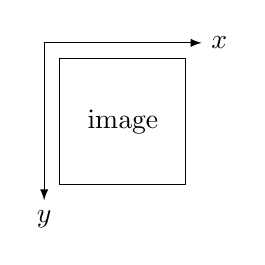
\begin{tikzpicture}[scale=2]
\draw[-latex] (0,0) -- (1,0);
\draw[-latex] (0,0) -- (0,-1);
\draw (0.1,-0.1) rectangle (0.9, -0.9);
\draw (0.5,-0.5) node {image};
\draw (1,0) node[right] {\(x\)};
\draw (0,-1) node[below] {\(y\)};
\end{tikzpicture}
\end{wrapfigure}

The frames are then read by openCV and converted into grey. OpenCV represents images with matrices whose indexes may also be seen as coordinate of the following base. An image pixel is then characterized by its coordinate in the following order: \verb|image[y,x]| (matrix line, matrix column).

We then apply a bilateral filter to the image, as it is a filter that preserve the sharp edges and smooth the rest of the image: this is exactly what we need, especially as there is a pattern with lines on the carpet of the Marconi amphiteater that needs to be removed.

% inserer capture de l'image filtree ?

After having a clear image of the line, we apply the Hough transform which will give us a set of straight lines detected on the image. But before calculating any angle, we need to reorient the lines accordingly to our purpose. Indeed, openCV will return us vectors that are oriented towards increasing \(x\), but we need to have them all in the same directon as \(y\), because the user moves on the y axis.

% place le ou tu veux comme tu veux Gui
\begin{tikzpicture}[scale=2]
  \draw[-latex] (0,-0.6) -- (0,-1.6);
  \draw (0,-1.6) node[below] {\(y\)};

  \draw (0.7,-0.3) -- (1.2,-1.1);
  \draw (1.2,-1.5) -- (0.7,-2.3);

  \draw[->] (1.4, -0.6) -- (1.6, -0.6);
  \draw[->] (1.4, -1.9) -- (1.6, -1.9);

  \draw[->] (2,-0.3) -- (2.5,-1.1);
  \draw[<-] (2.5,-1.5) -- (2,-2.3);

  \draw[->] (2.7, -1.9) -- (2.9, -1.9);

  \draw[->] (3.7,-1.5) -- (3.2,-2.3);
\end{tikzpicture}

Afterwards, we consider only the bottom of the frame and we compute the \textit{oriented} angle of each vector \(v_i\) with the \(y\) axis (defined as the \(\alpha\) angle), using:
\[ {\alpha}_i = \text{sgn}(x) \text{arcos}\left(\frac{y_i}{\|v_i\|}\right) \]
This angle is effectively the one that has our interest, since it is the same if we flip the vectors in the other direction along the \(y\) axis.
Then we calculate the average of the \(\alpha_i\) angles, which gives us our final \(\alpha\).

In the case the user is not on the line, we had the following strategy to get him back to it: we calculate the angle between the user and a target zone of the line where we want the person to go. As the evaluation is a race, and as a failure could not worsen anything by itself (we count the number of failures and not their durations), we put the target zone a little bit ahead of the line, so that the user gets back to it quickly. This angle has been called the \(\beta\) angle.

In order to compute it, we take a portion of the image vertically, and look at the barycentre of the pixels that were detected as an edge. Then we have a vector between the barycentre and the user (bottom middle horizontally), which angle with the \(y\) axis is computed the same way as for the \(\alpha_i\).

We have to know when to take the \(\beta\) angle into account. For this, we compute the distance between the user and the bottom of the line, parameter we call \(d\). The method is the same as for the target zone: we compute the barycentre of a portion of the pixels that were detected as edges, and then we just count the distance in pixels between the middle of the image and this barycentre (only along the \(x\) axis). 

% mettre les images des posters pour ces paragraphes ?? a toi de voir Guigz

If there is no line in the portion were we look for it, we then only take the \(beta\) angle into account, because that means that the user is very far from the line and should first get back to it. Otherwise, we mix the \(\alpha\) and the \(\beta\) angle relatively to the \(d\) parameter, so that the further the user is from the line, the more we take the second angle into account.

We use a \(d\)-dependant weight function, which is

\[ f(d) = (1 - e^{\frac{-d}{\tau}}) \]

We choose \(\tau\) so that when we are at the image extremity, the value of \(f\) is \(0.95\). Thus we have
\[ 3\tau = \frac{\text{width}}{2}, \quad \tau = \frac{\text{width}}{6} \]
It follows,
\[f(d) = 1 - e^{\frac{-6d}{w}}\]

Then, for the angle communicated to the user, called \(\gamma\), we choose this expression to have the behaviour we explained sooner.

\[ \gamma = (1 - f(d))\alpha + f(d)\beta \]

Hence we have,

\[ \gamma = \alpha + (1 - e^{\frac{-6d}{w}})(\beta - \alpha) \]

Before sending \(\gamma\) to the sound generation module, we bound the value of the angle in \([-70°, 70°]\). We also reserve \(\gamma = 100\) when no line is detected on the image. Then we send the angle.

\textit{Note:} would we have a cover to fix the raspberry on the body, could we better tune the position of the zones we look at, because we know the Raspberry's camera aperture, and giving the average height of a body, we know which distance we cover with camera and what pixel corresponds to what position in real life.

\subsection{Description of source files directory}

In the folder of the source code archive, you will find the \verb|rasp_prod| folder, containing the production source code for the raspberry device, the \verb|improc| and \verb|soundproc| folder containing our test codes for development, and the case folder containing some aborted concept protection and fixation covers for the raspberry. (...)

%------------- Commandes utiles ----------------

\section{Quelques commandes}

Voici quelques commandes utiles :

%------ Pour insérer et citer une image centralisée -----

\insererfigure{logos/EPL.jpg}{3cm}{Légende de la figure}{Label de la figure}
% Le premier argument est le chemin pour la photo
% Le deuxième est la hauteur de la photo
% Le troisième la légende
% Le quatrième le label
Ici, je cite l'image \ref{fig: Label de la figure}


%------- Pour insérer et citer une équation --------------

\begin{equation} \label{eq: exemple}
\rho + \Delta = 42
\end{equation}

L'équation \ref{eq: exemple} est cité ici. 

% ------- Pour écrire des variables ----------------------

Pour écrire des variables dans le texte, il suffit de mettre le symbole \$ entre le texte souhaité comme : constante $\rho$. 


\end{document}
